% !TEX program = xelatex
% FSE 2027 Research Papers: anonymous initial submission.
% Official CFP checked on 2026-09-07. Keep the class layout unchanged.
\documentclass[acmsmall,screen,review,anonymous]{acmart}

\usepackage{tabularx}
\usepackage{array}
\usepackage{multirow}

\setcopyright{none}
\settopmatter{printacmref=false}
% Review copy: omit unassigned rights and publication metadata.
% The original acmart typography, running heads, folios and line numbers remain.
\renewcommand\footnotetextcopyrightpermission[1]{}
\makeatletter
\AtBeginDocument{%
  \apptocmd{\ps@firstpagestyle}{\fancyfoot{}}{}{}
  \apptocmd{\ps@standardpagestyle}{\fancyfoot{}}{}{}
  \pagestyle{standardpagestyle}%
}
\makeatother
\acmDOI{}
\acmISBN{}
\acmYear{2027}
\copyrightyear{2027}
\acmConference[FSE 2027]{ACM International Conference on the Foundations of Software Engineering}{}{}
% Set the actual submission identifier when one has been assigned.
% \acmSubmissionID{...}

\title[Do Code Language Models Follow Tests?]{Do Code Language Models Follow Tests? Paired Interventions on Program Behavior}
\author{Anonymous Author(s)}
\newcommand{\QualityTasks}{180}
\newcommand{\QualityHE}{68}
\newcommand{\QualityMB}{112}
\newcommand{\QualityHighKill}{92.3}
\newcommand{\QualityLowKill}{62.0}
\newcommand{\QualityRandomKill}{91.3}


\begin{document}

\begin{abstract}
Tests express concrete requirements for generated programs, yet higher benchmark accuracy alone does not show whether a code language model adopts those requirements.
We study this distinction through paired semantic interventions that hold a task description and example inputs fixed while changing expected outputs between two valid rules.
Both generated programs must follow their assigned rules on unseen inputs, and explicit-rule prompts separately measure implementation capability.
Across five models, three runs, and 120 paired instances from 20 specification families, switching rates range from 11.1\% to 65.8\%.
Both 27B models implement every explicitly stated rule, but most of their test-conditioned failures follow the alternative rule.
Replaying displayed assertions shows that 97.3\% of hidden-rule failures already violate a visible example.
Matched experiments on 710 benchmark tasks find that correct outputs improve MBPP+ generation beyond inputs alone for every model, whereas gains vary across the other benchmarks.
On 180 tasks with fixed three-test suites, increasing fault detection by 30.3 percentage points changes generation accuracy by only $-0.6$ to $+1.1$ points.
Prompt representations respond to rule changes, but the tested linear probes have higher error than constant baselines on unseen families.
These findings identify a gap between implementing a rule and adopting it from tests, and show why test selection for generation needs evaluation beyond fault detection.

\end{abstract}

\ccsdesc[500]{Software and its engineering~Software testing and debugging}
\ccsdesc[300]{Software and its engineering~Automatic programming}
\keywords{code generation, language models, executable specifications, software testing, empirical study}

\maketitle

\section{Introduction}

Visible tests can resolve requirements that a short natural-language description leaves open.
Output order, endpoint inclusion, and tie breaking are common examples: two programs can satisfy the same description while disagreeing on a displayed assertion.
Test-driven prompting uses such examples as partial executable specifications, and prior work reports improvements in generated code \citep{mathews2024tdd,fakhoury2024ticoder}.
For software developers, the useful property is that the generated program follows the behavior specified by those examples.

Benchmark correctness combines several effects of adding tests.
Examples expose input formats, supply expected outputs, and may suggest a familiar implementation.
A higher pass rate therefore gives an incomplete account of which constraint the generator adopted.
Conversely, failure may arise from implementing an algorithm incorrectly even when the intended rule is explicit.
Requirements-clarification systems acquire missing intent through questions and answers \citep{li2023python,mu2024clarifygpt}.
We examine whether that intent, once expressed through test outputs, is reflected in the generated program.

Consider a request to remove duplicates from a list.
Preserving first-occurrence order and sorting the distinct values both satisfy this description.
We provide the same three input lists with outputs that specify one order or the other.
The model generates a separate program for each condition, and both programs are evaluated on unseen inputs.
A successful pair follows both assigned rules.
Explicit descriptions of the two rules provide a separate measure of the model's ability to implement them.
Figure~\ref{fig:paired-intervention} illustrates this intervention.

This design connects a change in the supplied specification to a change in program behavior.
We first measure rule adoption across 20 specification families and inspect how failures retain alternative conventions in code.
We then use matched benchmark prompts to separate expected outputs from input examples and conflicting constraints.
A fixed-budget test-selection experiment asks whether tests that detect more faulty programs also help a generator produce correct code.
Finally, representation analysis examines whether changes in prompt states track the observed rule adoption.

The experiments concern a single generation from the supplied prompt.
CodeT selects candidate solutions through test agreement, while Self-Debugging and AlphaCodium use feedback to revise programs \citep{chen2023codet,chen2024selfdebug,ridnik2024alphacodium}.
Our design examines the initial use of test-specified requirements before those selection and repair stages.

\begin{figure}[!htbp]
\centering
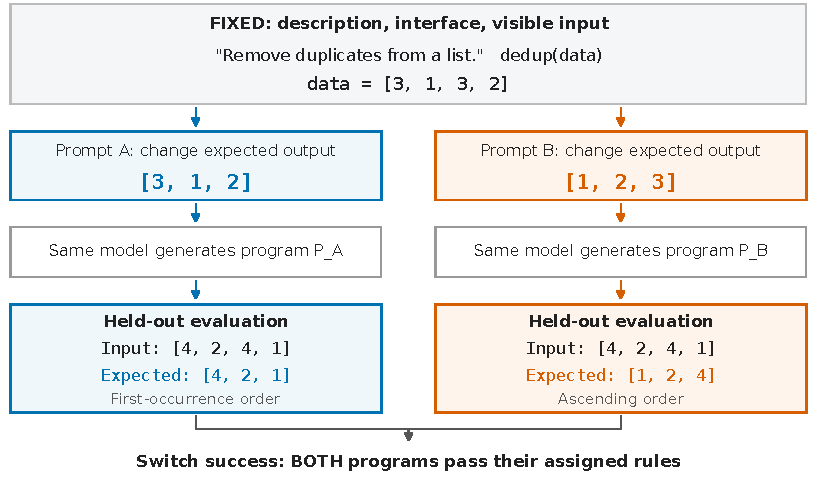
\includegraphics[width=\linewidth]{Figures/paired_intervention.pdf}
\caption{Paired semantic intervention, illustrated with duplicate removal. The description, function interface, visible inputs, and model are fixed; only expected outputs differ between A and B. One visible and one unseen input are shown for illustration. A successful switch requires both separately generated programs to follow their assigned rules over the full held-out evaluation suite.}
\label{fig:paired-intervention}
\Description{A fixed description and visible input branch into two prompts with different expected outputs. The same model generates separate programs for A and B. Both programs must follow their assigned rules on unseen inputs for the pair to count as a successful switch.}
\end{figure}

The central finding is a gap between implementing a rule and adopting it from tests.
Qwen3.6-27B and Qwen3.8-27B implement both explicitly stated rules throughout the paired tasks, yet their mean switching rates under tests are 60.6\% and 65.8\%.
Most of their failed outputs implement the alternative rule, with endpoint comparisons and case normalization providing concrete examples.
Replaying the displayed assertions further shows that most hidden-rule failures are already observable on the examples supplied to the model.

The study contributes a controlled way to measure this adoption gap and an empirical account of where it appears in generated programs.
The benchmark controls show when expected outputs contribute beyond example inputs and how conflicting tests affect correctness.
The fixed-size suite experiment separates the utility of tests for checking programs from their utility for generating them.
Together, these results give code-generation evaluators and test-selection researchers distinct behavioral outcomes to measure: implementing a rule, adopting a test-specified rule, and producing correct code.

\section{Study Design}

We study test utilization at three levels: adoption of a specified rule, correctness on programming benchmarks, and the generation utility of selected tests.
The paired experiment supplies the direct behavioral measure; the other two experiments examine its relationship to conventional correctness and testing criteria.

\subsection{Paired Semantic Interventions}

We author 20 specification families covering ordering, duplicate handling, tied optima, interval boundaries, arithmetic conventions, string matching, grouping, and graph reachability.
Each family defines two reference implementations, A and B, and a description that leaves their distinguishing rule open.
The function signature and input containers are explicit.
For example, a substring task receives the two-element list containing the text and pattern under both rules.

Table~\ref{tab:semantic-rules} lists the alternative rules for each family.
\begin{table}[!htbp]
\centering
\caption{Alternative rules used in the semantic intervention. Each pair shares an underspecified description, function signature, and three visible inputs. The explicit conditions add the corresponding rule to the description.}
\label{tab:semantic-rules}
\small
\begin{tabularx}{\linewidth}{@{}>{\raggedright\arraybackslash}p{.18\linewidth}>{\raggedright\arraybackslash}X>{\raggedright\arraybackslash}X@{}}
\toprule
Family & Rule A & Rule B \\
\midrule
dedup order & Preserve the order of first occurrence. & Return the distinct integers in ascending order. \\
duplicate policy & Keep the first occurrence of each value. & Keep only values that occur exactly once in the input. \\
argmax tie & Choose the first such index. & Choose the last such index. \\
threshold boundary & Include values equal to the threshold. & Include only values strictly greater than the threshold. \\
interval boundary & Include both bounds. & Include the lower bound and exclude the upper bound. \\
median choice & For even-length lists choose the lower middle value. & For even-length lists choose the upper middle value. \\
integer rounding & Round the quotient down toward negative infinity. & Truncate the quotient toward zero. \\
remainder sign & Use the nonnegative remainder associated with floor division. & Use the signed remainder associated with truncation toward zero. \\
substring overlap & Count overlapping occurrences. & Count non-overlapping occurrences from left to right. \\
substring case & Match letters case-sensitively. & Match letters case-insensitively. \\
space fields & Consecutive spaces separate empty fields; preserve leading and trailing empty fields. & Treat consecutive spaces as one separator and omit empty fields. \\
normalization & Keep decimal digits as part of the normalized text. & Keep alphabetic letters only. \\
sort ties & Preserve input order among equal scores. & Sort equal scores by ascending name. \\
partial chunk & Keep the final chunk even when it is shorter than the requested size. & Return only chunks of the full requested size. \\
group count & Group consecutive equal values into runs. & Group all occurrences of each value together. \\
graph direction & Each edge can be traversed from u to v only. & Each edge can be traversed in either direction. \\
merge touching & Also merge intervals whose endpoints touch. & Merge intervals only when their interiors overlap. \\
search index & The first position is numbered zero. & The first position is numbered one. \\
topk ties & Return exactly k values. & Include every value equal to the cutoff, even when the result has more than k elements. \\
empty segments & Keep entries that are empty after trimming. & Discard entries that are empty after trimming. \\
\bottomrule
\end{tabularx}

\end{table}


Each family has six realizations with distinct input sets, giving 120 paired instances.
We sample three visible inputs on which A and B disagree.
The A-test and B-test prompts contain these same inputs and the corresponding reference outputs.
Both prompts present the problem description, function signature, and visible assertions in that order, followed by an answer section.
The final instruction is ``Return a complete Python implementation inside a Python markdown block.''
The artifact includes the complete prompts used for every instance.
We also generate programs from NL-only, inputs-only, and descriptions that state A or B explicitly.
The explicit conditions measure whether the model can implement the rule when it is supplied directly in language.
They provide the complete distinguishing rule as an oracle clarification, making its implementation directly observable alongside the response to tests.

Evaluation uses 30 new distinguishing inputs per instance.
For families with inputs on which both references agree, we additionally sample up to ten such inputs and require the program to pass them.
Visible and evaluation inputs are disjoint across the six realizations of a family.
We classify a program as following A or B only if it passes every input for that rule.
A program may follow neither rule.
We also replay each A/B-test program on its three displayed assertions and cross-tabulate visible adherence with hidden-rule outcomes.
These counts describe repeated generation records from the same 120 instances.

Our primary metric is \emph{paired rule switching}: the fraction of instances for which the A-test program follows A and the B-test program follows B.
This joint requirement measures whether changing only the output constraints changes the generated behavior in the requested direction.
We also report A and B adherence separately, together with the default behavior under NL-only and inputs-only prompting.
We compute this joint outcome within each instance and run, then average the three outcomes within the instance.
We report both the aggregate switching rate and the distribution across specification families.

\subsection{Matched Benchmark Prompts}

For each task, four core prompts share the same problem description and function interface.
\textbf{NL-only} contains the description alone.
\textbf{Correct I/O} adds public inputs and their expected outputs.
\textbf{Wrong I/O} retains those inputs and changes the expected outputs while preserving their data types.
\textbf{Inputs-only} supplies the same inputs without outputs.
The distinction between inputs and expected outputs reflects the test-oracle problem: exercising a program and specifying its correct behavior provide different information \citep{barr2015oracle}.
We remove example blocks from the description before constructing the four conditions.
Function tasks expose up to three public examples; LiveCodeBench uses each task's official public examples.
The retained count is identical across the three example conditions for each task.

Function-task outputs are evaluated against the reference implementation.
Every correct assertion must pass, and every modified output must fail that implementation.
A value without a supported type-preserving corruption, such as \texttt{None}, remains unchanged when another output in the same suite can be changed.
We record the number of changed outputs for each task.
LiveCodeBench corruptions change the official expected stdout or return value without changing the public input or calling convention.
Thus, the wrong-output condition measures response to conflicting evidence; the paired intervention measures response to compatible alternative specifications.
The inputs-only comparison measures what expected outputs add to the prompt.
Wrong outputs probe the response to conflicting constraints while keeping the target inputs and interface fixed.


\paragraph{Tests from other tasks.}
An additional \textbf{Other-task} condition supplies tests that are correct for a different source task, using the same test-block format as correct I/O.
The donor mapping is fixed across all five models and three runs.
Function tests use the current function name and preserve argument count, with preference for matching input and output structure types and test length.
LiveCodeBench donors preserve the calling convention.
For two tasks with unique four-argument interfaces, independently authored source tasks provide the donor tests; their reference implementations are retained.
Donor inputs overlap neither the target task's visible inputs nor its evaluation inputs, so all five conditions use the same held-out evaluation set.

Of 2062 displayed tests, 1817 exactly match the original input structure type and 1715 match the output structure type.
The median donor-to-original length ratio is 1.0, with 1729 tests within $\pm15\%$ of the original length.
On the 535 function-task references, 11 donor suites happen to pass completely and 68 produce an execution error or timeout.
The remaining mismatches and accidental passes are retained in the control audit.
Correct-minus-other-task measures the advantage of task-specific correct examples over these donor examples; other-task-minus-NL measures the net effect of adding donor tests.
Because donor tests may impose incorrect constraints on the target, these contrasts combine content relevance and interference rather than isolating a pure text-length or formatting effect.

\subsection{Selecting Tests by Fault Detection}

The quality experiment uses \QualityTasks{} HumanEval+/MBPP+ tasks with reference implementations.
For each task, we retain at least five distinct candidate inputs from the generated test pool and execute every candidate assertion against the reference.
The original public examples form a development set for identifying faulty programs.
We collect erroneous generated programs and single-edit AST mutants of the reference, requiring successful initialization and at least one failure on the development set.
These mutants supply a fault-based measure of test strength \citep{jia2011mutation}; the independent validation pool measures detection beyond the errors used for selection.

We form a selection pool and a separate validation pool, each containing three to eight erroneous programs.
The pools use different mutation-operator families and contain no identical programs after AST normalization.
Selection mutations include arithmetic, aggregation, loop bounds, ordering parameters, and omitted filters.
Validation mutations include comparisons, constant boundaries, parameter substitutions, and input slices.
Generated programs augment these pools; their development-set behavior determines eligibility.
Across the 180 tasks, the selection pools contain 1088 erroneous programs, including 162 generated programs, and the validation pools contain 1236, including four generated programs.
The remaining programs are reference mutants.
All program sources and per-test outcomes are retained with the task.

For a suite of three tests, fault detection is the fraction of pool programs that fail at least one test in the suite.
This union criterion rewards complementary tests rather than repeatedly detecting the same error.
We enumerate the three-test combinations, restricting total assertion length to within 15\% of the median combination length.
The highest- and lowest-detection suites are selected using the selection pool, and a random suite is sampled from the same feasible combinations.
A task enters the experiment when a high-versus-low contrast exists in the selection pool.
The validation pool is then used to measure the detection rates of the selected suites; it does not determine selection or task inclusion.

We generate one program from each of four prompts: NL-only, random three tests, low-detection three tests, and high-detection three tests.
Final evaluation excludes every candidate-pool input and every development input, including candidates that were never displayed.
The two primary contrasts compare the high-detection suite with the random and low-detection suites.
We measure the detection contrast on the held-out error pool and estimate the paired generation difference on the final evaluation inputs.

\section{Experimental Setup}

\subsection{Benchmarks and Models}

The source benchmark collection contains 164 HumanEval+ tasks, 378 MBPP+ tasks, and 175 LiveCodeBench v6-new tasks.
HumanEval+ and MBPP+ extend the original benchmarks with more extensive functional tests \citep{chen2021codex,austin2021mbpp,liu2023evalplus}.
LiveCodeBench v6-new is the difference between releases v6 and v5, containing 43 easy, 52 medium, and 80 hard problems from AtCoder and LeetCode \citep{jain2024livecodebench}.
The matched protocol contains 710 tasks: 157 HumanEval+, 378 MBPP+, and all 175 LiveCodeBench tasks.
Seven HumanEval tasks lack a public example that the direct-call construction can materialize; their identifiers and reasons accompany the dataset.

All three experiments use five checkpoints: Qwen2.5-Coder-7B-Instruct \citep{hui2024qwen25coder}, Qwen3.5-9B \citep{qwen35model}, Qwen3.6-27B \citep{qwen36}, Qwen3.8-27B \citep{qwen38model}, and DeepSeek-Coder-6.7B-Instruct~\citep{guo2024deepseek}.
Tables abbreviate the first and last names as Qwen2.5-7B and DeepSeek-6.7B.
The controlled experiments comprise 67,650 generations: 53,250 in the main experiment, 10,800 in the semantic experiment, and 3600 in the quality experiment.
The main experiment includes 10,650 other-task generations and reuses the 42,600 completed generations for the four core conditions.
All controlled generations use native chat templates, BF16 weights, greedy decoding, an 8192-token output budget, and a 16384-token context limit in vLLM 0.25.1.
Thinking is disabled for Qwen3.5, Qwen3.6, and Qwen3.8; all inputs are text.
Qwen3.8 main-experiment generation is partitioned into three request ranges with two-way tensor parallelism; the ranges retain the original batch boundaries.
The recorded execution settings accompany each experiment.
We retain complete generated solutions, including helper functions and executable entry points.

\subsection{Evaluation and Repeated Runs}

We report two correctness labels for benchmark tasks.
The complete official label uses all available benchmark tests.
The primary held-out label removes the inputs exposed through the prompt; in the quality experiment it removes the entire candidate and development input pools.
Aligned input and expected-output arrays are filtered together, while the benchmark's comparison function is preserved.
All 535 function-task references pass both versions of the main evaluator.
Function suites use a 15-second budget, extended to 60 seconds for the task whose reference repeatedly sums long integer ranges.
Visible-suite replay used Python 3.12.14, while held-out labels came from Python 3.12.13; 11 DeepSeek programs timed out under the shared 15-second budget and count as visible failures.
LiveCodeBench uses its official checker with the full suite and with private inputs that do not duplicate public inputs.
Each LiveCodeBench worker has a 4\,GiB address-space budget and a 15-second per-test time limit.
The same checker handles standard-input programs and function-call tasks.

Each main and semantic condition is executed three times, with the generation seed fixed and task order varied across runs.
These repetitions measure stability under greedy inference and batch scheduling.
For each contrast, we average its paired correctness difference over the three runs within a task.
The sample size remains the number of tasks: three LiveCodeBench runs evaluate the same 175 tasks.
We report per-run effects alongside their means to show whether the direction of a contrast persists across executions.
Semantic results retain the grouping into 20 specification families, each with six realizations.
The quality experiment uses one generation per condition and task, and reports paired gains and losses where they explain the aggregate difference.

\section{Behavioral Results}

\subsection{Rule Adoption and Implementation Capability}

Both 27B models implement every explicitly stated rule, yet adopt test-specified alternatives less consistently (Table~\ref{tab:semantic}).
Qwen3.8 follows A in 95.6\% of A-test instances and B in 70.3\% of B-test instances, with a paired switching rate of 65.8\%.
Qwen3.6 reaches 92.5\% A adherence, 66.9\% B adherence, and 60.6\% paired switching.
The explicit-rule controls succeed in every run, so the failed test-conditioned outputs concern rules these checkpoints can implement.

The same distinction appears in Qwen3.5: B adherence is 32.5\% under tests and 88.6\% under an explicit description, while paired switching reaches 24.2\%.
Qwen2.5 and DeepSeek each switch in 11.1\% of instances.
DeepSeek's explicit A/B scores of 68.9\% and 43.3\% show a further constraint on its performance: some rules remain difficult even when stated directly.

\begin{table}[!htbp]
\centering
\caption{Rule adherence and paired switching (\%) averaged over three runs of 120 paired instances from 20 specification families. Tests A/B and Explicit A/B are scored against the assigned rule; NL-only columns report the default rule distribution. Switching requires successful A and B programs on the same instance and run.}
\label{tab:semantic}
\small
\begin{tabular}{crrrrrrr}
\toprule
Model & NL: A & NL: B & Tests A & Tests B & Explicit A & Explicit B & Paired switch \\
\midrule
Qwen2.5-7B & 70.8 & 10.0 & 73.9 & 21.1 & 84.4 & 65.0 & 11.1 \\
Qwen3.5-9B & 89.2 & 5.8 & 88.1 & 32.5 & 100.0 & 88.6 & 24.2 \\
Qwen3.6-27B & 70.0 & 25.0 & 92.5 & 66.9 & 100.0 & 100.0 & 60.6 \\
Qwen3.8-27B & 81.4 & 14.7 & 95.6 & 70.3 & 100.0 & 100.0 & 65.8 \\
DeepSeek-6.7B & 70.0 & 5.8 & 65.3 & 31.7 & 68.9 & 43.3 & 11.1 \\
\bottomrule
\end{tabular}
\end{table}


Input-only prompts identify the contribution of expected outputs.
For Qwen3.8, B adherence rises from 21.1\% with inputs alone to 70.3\% with B tests, an increase of 49.2 points.
The corresponding increase is 42.8 points for Qwen3.6 and 15.0 points for DeepSeek.
Expected outputs therefore change which rule the generated program follows, while the joint switching metric additionally requires successful A and B programs on the same instance and run.

The deduplication family makes this response visible in code.
For one realization in the first run, Qwen2.5 generates \texttt{list(set(data))} under both test conditions, satisfying neither required order on the held-out inputs.
Qwen3.6 generates a traversal that tracks previously seen values under A tests and \texttt{sorted(set(data))} under B tests.
Figure~\ref{fig:semantic-families} shows how these outcomes vary across all families.
Qwen3.8 switches on all six realizations in every run for nine families and never switches for three; Qwen3.6 has seven complete-success families and four zero-switch families.
Their explicit-rule controls succeed across all of these families.

Aggregate switching rates change little across the three runs (Table~\ref{tab:semantic-repeats}).
Qwen3.8 ranges from 65.0\% to 66.7\%, and Qwen3.6 from 60.0\% to 60.8\%.
The family breakdown exposes a larger behavioral contrast: persistent success on some conventions and persistent failure on others.
These repetitions describe execution stability on the same instances.

\begin{figure}[!htbp]
\centering
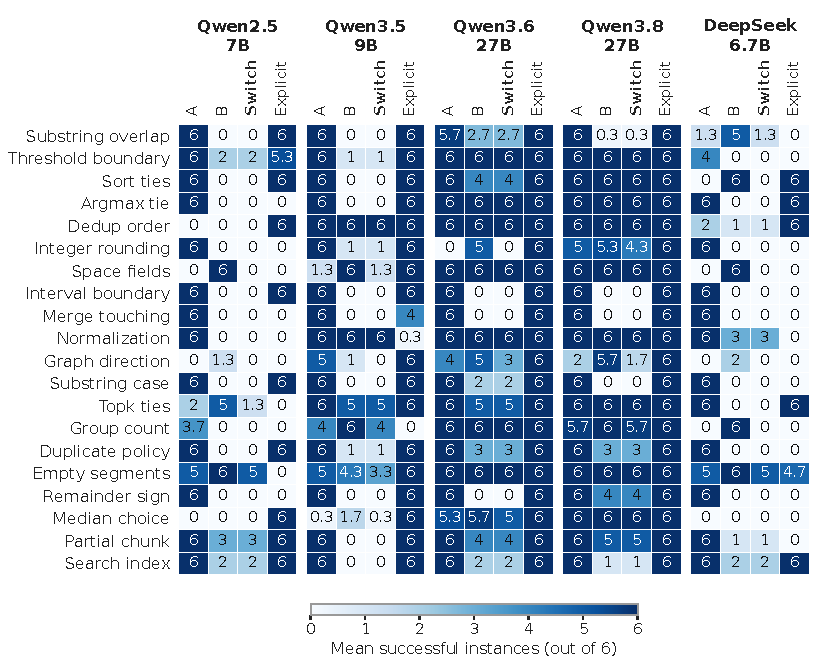
\includegraphics[width=\linewidth]{Figures/semantic_families_heatmap.pdf}
\caption{Mean successful instances per run within each specification family, out of six. Color and cell labels show values averaged over three runs. A and B score the corresponding test-conditioned program. Switch and Explicit require successful A and B programs for the same instance and run under tests and explicit rules, respectively. All model panels use the same 0--6 scale.}
\label{fig:semantic-families}
\Description{Five annotated heatmaps show 20 specification families for Qwen2.5, Qwen3.5, Qwen3.6, Qwen3.8, and DeepSeek. Each model has A, B, Switch, and Explicit columns, with rounded means printed in every cell on a shared scale from zero to six.}
\end{figure}
\begin{table}[!htbp]
\centering
\caption{Paired rule switching (\%) in each run on the same 120 instances from 20 families. Full per-run adherence results are retained in the replication materials.}
\label{tab:semantic-repeats}
\small
\begin{tabular}{crrr}
\toprule
Model & Run 1 & Run 2 & Run 3 \\
\midrule
Qwen2.5-7B & 10.8 & 11.7 & 10.8 \\
Qwen3.5-9B & 24.2 & 25.0 & 23.3 \\
Qwen3.6-27B & 60.8 & 60.8 & 60.0 \\
Qwen3.8-27B & 65.8 & 66.7 & 65.0 \\
DeepSeek-6.7B & 10.8 & 10.8 & 11.7 \\
\bottomrule
\end{tabular}
\end{table}


\subsection{Visible Adherence and Persistent Rule Failures}
\label{sec:behavior-failures}

\paragraph{Failures already exposed by the prompt.}
Across the 3,600 A/B-test generations, 2,331 pass all three displayed assertions and 2,296 pass the assigned hidden rule.
Every hidden-rule success also passes the displayed assertions.
Of 1,304 hidden-rule failures, 1,269 (97.3\%) fail at least one displayed assertion; the other 35 pass the examples but fail both hidden rules.
Most observed failures therefore occur before the distinction between fitting the examples and generalizing beyond them becomes relevant.

\paragraph{Retaining the rule observed without tests.}
Among task-run records where NL-only follows A, B tests yield B in 21.2\% (54/255) for Qwen2.5, 28.3\% (91/321) for Qwen3.5, 56.7\% (143/252) for Qwen3.6, 64.5\% (189/293) for Qwen3.8, and 25.0\% (63/252) for DeepSeek.
This conditional transition measures whether B tests change the behavior observed without examples.
Paired switching additionally requires successful implementation of A under A tests.

A failed paired switch can arise because a program adopts the other rule or because it satisfies neither rule.
Table~\ref{tab:representation-diagnosis} separates these outcomes over the 720 A/B-test completions per model.
Among Qwen3.6's 146 completions that fail the target rule, 139 (95.2\%) pass the other rule; for Qwen3.8, the corresponding count is 119 of 123 (96.7\%).
Thus, these models' target-rule failures predominantly implement the alternative behavior rather than fail both specifications.
These descriptive proportions count repeated generation records from the same paired instances.

\begin{table}[!htbp]
\centering
\caption{Behavioral categories over 720 existing completions per model. Target and Other pass the corresponding rule; Neither passes neither. The last three columns partition Neither into initialization/runtime errors (Error), mismatches on shared inputs (Shared), and remaining rule-output mismatches (Remaining). Counts include three runs of the 240 A/B prompts per model.}
\label{tab:representation-diagnosis}
\small
\setlength{\tabcolsep}{3pt}
\begin{tabular}{crrrrrr}
\toprule
Model & Target & Other & Neither & Error & Shared & Remaining \\
\midrule
Qwen2.5-7B & 342 & 277 & 101 & 29 & 36 & 36 \\
Qwen3.5-9B & 434 & 233 & 53 & 0 & 19 & 34 \\
Qwen3.6-27B & 574 & 139 & 7 & 1 & 3 & 3 \\
Qwen3.8-27B & 597 & 119 & 4 & 0 & 1 & 3 \\
DeepSeek-6.7B & 349 & 259 & 112 & 37 & 33 & 42 \\
\bottomrule
\end{tabular}
\end{table}


\paragraph{Persistent failures on specific conventions.}
We inspect Qwen3.8's three zero-switching families in Figure~\ref{fig:semantic-families}: interval boundaries, merging touching intervals, and substring case handling.
Across their 18 instances and three runs, NL-only produces rule A in all 54 records.
B tests produce A in 51 records and neither rule in three, while explicit B succeeds in all 54.
The three neither-rule outcomes belong to interval boundaries.
In these families, most B-test programs therefore retain the rule observed without tests despite outputs that distinguish B.

For interval boundaries, one displayed input has values $[-3,-2,1,-3,-1,-3,-1]$, lower bound $-3$, and upper bound $-1$.
Its B output is $[-3,-2,-3,-3]$, excluding the upper endpoint.
For instance 0 in the first run, both NL-only and B tests yield \texttt{lo <= x <= hi}; the explicit-B program uses \texttt{lo <= x < hi}.
The B-test program consequently includes the two $-1$ values and fails the displayed constraint as well as the held-out rule.

The other families expose analogous local implementation choices.
For merging touching intervals, the first instance's B-test program merges when \texttt{interval[0] <= last[1]}, although B examples keep touching endpoints separate; explicit B uses strict overlap comparisons.
For substring matching, a visible B assertion requires six matches of \texttt{'Ab'} in \texttt{'AbABAbababAB'}.
The B-test program searches the original strings with \texttt{text.find}, finding two case-sensitive matches, while the explicit-B program lowercases both strings and returns six.
These examples locate the behavioral mismatch in concrete comparisons and normalization operations.
They do not reflect uniformly poor performance on all conventions: Qwen3.8 switches completely for deduplication order, argmax ties, and sort ties.

\paragraph{Programs satisfying neither rule.}
Across all models, 277 records pass neither rule.
Per-test replay preserves every original category and separates initialization or runtime errors, mismatches on inputs shared by both rules, and remaining rule-specific output mismatches.
The four Qwen models contribute 165 such records involving 52 distinct programs; DeepSeek contributes 112 records.
A shared-input mismatch indicates failure of common functionality, while instances without shared inputs leave that functionality unobserved.
The remaining category records unmet rule outputs without inferring program intent.

\subsection{Expected Outputs and Benchmark Correctness}

Expected outputs improve correctness beyond input examples on MBPP+ for all five models, while their benefit varies on HumanEval+ and LiveCodeBench.
Table~\ref{tab:main} reports mean held-out pass rates over three runs on the same 157 HumanEval+, 378 MBPP+, and 175 LiveCodeBench tasks.
Figure~\ref{fig:main-effects} contrasts correct I/O with NL-only, inputs-only, and wrong I/O; each difference averages paired task outcomes across the three runs.
Table~\ref{tab:repeats} retains the individual-run correct-minus-input-only effects.
Table~\ref{tab:unrelated} adds the other-task condition on the same tasks and held-out inputs.
Complete official-suite scores are retained in the replication materials.

\begin{table}[!htbp]
\centering
\caption{Held-out pass rates (\%), averaged over three runs. Exposed inputs are removed from the evaluation suite. Each task contributes one mean correctness value.}
\label{tab:main}
\small
\begin{tabular}{clrrrr}
\toprule
Model & Dataset & NL-only & Correct I/O & Wrong I/O & Inputs-only \\
\midrule
\multirow{3}{*}{Qwen2.5-7B} & HumanEval+ & 82.8 & 81.5 & 70.1 & 82.4 \\
& MBPP+ & 66.3 & 73.7 & 63.9 & 69.0 \\
& LCB v6-new & 23.4 & 21.9 & 19.4 & 20.6 \\
\addlinespace[2pt]
\multirow{3}{*}{Qwen3.5-9B} & HumanEval+ & 82.8 & 83.7 & 74.1 & 82.4 \\
& MBPP+ & 66.2 & 76.1 & 61.8 & 68.6 \\
& LCB v6-new & 39.4 & 40.0 & 33.5 & 38.9 \\
\addlinespace[2pt]
\multirow{3}{*}{Qwen3.6-27B} & HumanEval+ & 91.5 & 94.1 & 68.8 & 92.1 \\
& MBPP+ & 72.2 & 79.7 & 48.6 & 76.2 \\
& LCB v6-new & 56.4 & 54.3 & 51.2 & 56.6 \\
\addlinespace[2pt]
\multirow{3}{*}{Qwen3.8-27B} & HumanEval+ & 89.6 & 94.3 & 64.3 & 91.1 \\
& MBPP+ & 70.9 & 79.5 & 47.4 & 74.5 \\
& LCB v6-new & 53.1 & 54.1 & 43.4 & 52.6 \\
\addlinespace[2pt]
\multirow{3}{*}{DeepSeek-6.7B} & HumanEval+ & 72.8 & 72.2 & 64.1 & 69.0 \\
& MBPP+ & 60.4 & 69.3 & 60.8 & 64.0 \\
& LCB v6-new & 14.7 & 14.1 & 13.1 & 16.4 \\
\bottomrule
\end{tabular}
\end{table}

\begin{figure}[!htbp]
\centering
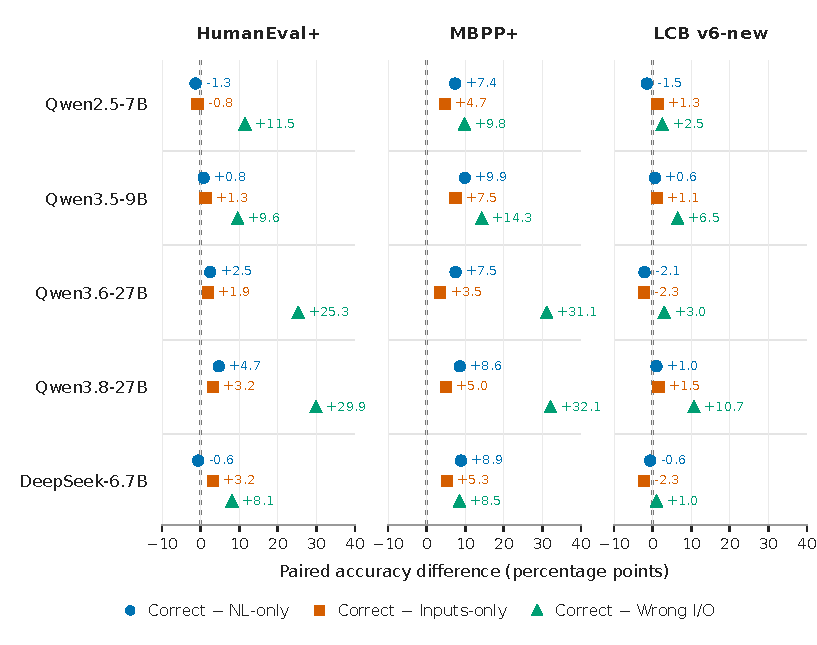
\includegraphics[width=\linewidth]{Figures/main_effects_forest.pdf}
\caption{Mean paired accuracy differences in percentage points. Points compare correct I/O with NL-only, inputs-only, and wrong I/O on each dataset. Repeated runs are averaged within tasks. The three dataset panels compare all five models on the same horizontal scale; dashed vertical lines mark zero difference.}
\label{fig:main-effects}
\Description{Three dataset panels display 45 mean paired accuracy differences across HumanEval+, MBPP+, and LiveCodeBench. Colors and marker shapes distinguish the three prompting contrasts. Every panel uses the same scale and includes a zero reference line.}
\end{figure}

\paragraph{Expected outputs add value on MBPP+.}
Correct I/O outperforms inputs-only for all five models, by 4.7 points for Qwen2.5, 7.5 for Qwen3.5, 3.5 for Qwen3.6, 5.0 for Qwen3.8, and 5.3 for DeepSeek.
Every model has a positive difference in each individual run.
Qwen3.5 illustrates the contribution of each prompt component: accuracy rises from 66.2\% with NL-only to 68.6\% with inputs alone and 76.1\% with correct I/O.
The recurring gain comes from expected outputs beyond the examples' input information.

\paragraph{The benefit depends on the task distribution.}
On HumanEval+, Qwen3.8 reaches 94.3\% with correct I/O, compared with 89.6\% under NL-only and 91.1\% under inputs-only.
Its paired gains are 4.7 and 3.2 points, respectively.
Correct-minus-input-only effects range from $-0.8$ to $+3.2$ points across the five models, compared with $+3.5$ to $+7.5$ on MBPP+.
On LiveCodeBench, they are $+1.3$, $+1.1$, $-2.3$, $+1.5$, and $-2.3$ points for Qwen2.5, Qwen3.5, Qwen3.6, Qwen3.8, and DeepSeek.
The smaller effects also change direction across runs for the two 27B models: Qwen3.8 records $+5.1$, $+2.3$, and $-2.9$ points, and Qwen3.6 records $-5.7$, $+1.1$, and $-2.3$.
High switching performance on the paired tasks thus coexists with uneven gains on general programming problems.

\paragraph{Incorrect outputs redirect generation.}
Wrong I/O lowers accuracy relative to correct I/O on both function benchmarks for every model.
Qwen3.8 loses 29.9 points on HumanEval+ and 32.1 on MBPP+; Qwen3.6 loses 25.3 and 31.1 points.
The same checkpoints that adopt alternative rules relatively often are also sensitive to incorrect expected outputs.
Outputs can influence generation in a harmful direction when their constraints conflict with the task.

\begin{table}[!htbp]
\centering
\caption{Per-run paired held-out differences (percentage points). Each cell lists Run 1 / Run 2 / Run 3. The same tasks are evaluated in every run; repetitions do not increase the independent sample size. Task-level gains, losses, and exact McNemar tests accompany the results.}
\label{tab:repeats}
\small
\begin{tabular}{cllll}
\toprule
Model & Dataset & Correct $-$ NL & Correct $-$ Inputs & Correct $-$ Wrong \\
\midrule
\multirow{3}{*}{Qwen2.5-7B} & HumanEval+ & -1.3 / -1.9 / -0.6 & -0.6 / -1.3 / -0.6 & +11.5 / +10.8 / +12.1 \\
& MBPP+ & +7.4 / +7.4 / +7.4 & +4.8 / +4.5 / +4.8 & +9.8 / +9.5 / +10.1 \\
& LCB v6-new & -1.1 / -0.6 / -2.9 & +1.7 / +1.7 / +0.6 & +2.9 / +2.9 / +1.7 \\
\addlinespace[2pt]
\multirow{3}{*}{Qwen3.5-9B} & HumanEval+ & +1.3 / +0.0 / +1.3 & +3.2 / -1.9 / +2.5 & +8.9 / +8.3 / +11.5 \\
& MBPP+ & +9.3 / +9.8 / +10.6 & +6.9 / +7.4 / +8.2 & +13.8 / +14.3 / +14.8 \\
& LCB v6-new & +1.7 / +1.7 / -1.7 & -1.1 / +4.0 / +0.6 & +5.7 / +4.6 / +9.1 \\
\addlinespace[2pt]
\multirow{3}{*}{Qwen3.6-27B} & HumanEval+ & +2.5 / +1.9 / +3.2 & +1.9 / +2.5 / +1.3 & +25.5 / +24.8 / +25.5 \\
& MBPP+ & +7.4 / +7.4 / +7.7 & +3.7 / +3.4 / +3.4 & +31.5 / +31.0 / +31.0 \\
& LCB v6-new & -5.7 / +0.0 / -0.6 & -5.7 / +1.1 / -2.3 & +1.7 / +4.0 / +3.4 \\
\addlinespace[2pt]
\multirow{3}{*}{Qwen3.8-27B} & HumanEval+ & +5.1 / +4.5 / +4.5 & +4.5 / +1.9 / +3.2 & +29.3 / +31.2 / +29.3 \\
& MBPP+ & +9.0 / +9.0 / +7.9 & +5.6 / +5.6 / +4.0 & +32.8 / +32.0 / +31.5 \\
& LCB v6-new & +1.7 / +4.6 / -3.4 & +5.1 / +2.3 / -2.9 & +9.1 / +12.0 / +10.9 \\
\addlinespace[2pt]
\multirow{3}{*}{DeepSeek-6.7B} & HumanEval+ & -1.3 / +0.0 / -0.6 & +3.2 / +3.8 / +2.5 & +8.3 / +9.6 / +6.4 \\
& MBPP+ & +9.0 / +9.0 / +8.7 & +5.0 / +5.6 / +5.3 & +8.7 / +8.5 / +8.2 \\
& LCB v6-new & -0.6 / -1.1 / +0.0 & -2.3 / -2.3 / -2.3 & +1.1 / +0.6 / +1.1 \\
\bottomrule
\end{tabular}
\end{table}



\paragraph{Response to tests from other tasks.}
Donor tests reduce accuracy relative to NL-only on both HumanEval+ and MBPP+ for every model (Table~\ref{tab:unrelated}).
The penalties range from 10.8 to 20.4 points on HumanEval+ and from 7.0 to 30.3 on MBPP+, with the same direction in every run.
Correct I/O outperforms donor tests by 9.6--25.1 points on HumanEval+ and 15.9--39.0 on MBPP+, again in every run.
Qwen3.8 has the largest decreases: NL-only accuracy falls from 89.6\% to 69.2\% on HumanEval+ and from 70.9\% to 40.6\% on MBPP+ after adding donor tests.
On LiveCodeBench, its donor condition is 7.4 points below NL-only and 8.4 points below correct I/O.

The test-block format alone does not make these examples useful to the generator.
Donor constraints can conflict with the target task, so correct-minus-donor includes both the contribution of relevant outputs and the harm caused by incompatible ones.
Inputs-only supplies the comparison for the added value of target outputs; wrong-output and other-task prompts reveal two forms of conflicting evidence.

\begin{table}[!htbp]
\centering
\caption{Tests from other tasks under the same three-run protocol. Other-task is held-out pass rate (\%); contrasts are percentage points. Correct I/O and NL-only reuse the runs in Table~\ref{tab:main}. Differences are computed before rounding.}
\label{tab:unrelated}
\small
\setlength{\tabcolsep}{4pt}
\begin{tabular}{clrrr}
\toprule
Model & Dataset & Other-task & Correct $-$ Other & Other $-$ NL \\
\midrule
\multirow{3}{*}{Qwen2.5-7B} & HumanEval+ & 72.0 & $+9.6$ & $-10.8$ \\
& MBPP+ & 53.9 & $+19.8$ & $-12.4$ \\
& LCB & 21.0 & $+1.0$ & $-2.5$ \\
\addlinespace[2pt]
\multirow{3}{*}{Qwen3.5-9B} & HumanEval+ & 69.2 & $+14.4$ & $-13.6$ \\
& MBPP+ & 49.7 & $+26.4$ & $-16.5$ \\
& LCB & 37.1 & $+2.9$ & $-2.3$ \\
\addlinespace[2pt]
\multirow{3}{*}{Qwen3.6-27B} & HumanEval+ & 76.4 & $+17.6$ & $-15.1$ \\
& MBPP+ & 43.0 & $+36.7$ & $-29.2$ \\
& LCB & 53.7 & $+0.6$ & $-2.7$ \\
\addlinespace[2pt]
\multirow{3}{*}{Qwen3.8-27B} & HumanEval+ & 69.2 & $+25.1$ & $-20.4$ \\
& MBPP+ & 40.6 & $+39.0$ & $-30.3$ \\
& LCB & 45.7 & $+8.4$ & $-7.4$ \\
\addlinespace[2pt]
\multirow{3}{*}{DeepSeek-6.7B} & HumanEval+ & 59.0 & $+13.2$ & $-13.8$ \\
& MBPP+ & 53.4 & $+15.9$ & $-7.0$ \\
& LCB & 15.4 & $-1.3$ & $+0.8$ \\
\bottomrule
\end{tabular}
\end{table}


\subsection{Fault Detection and Generation Utility}

The quality experiment holds the number of displayed tests at three while changing how they are selected.
Its \QualityTasks{} tasks comprise \QualityHE{} HumanEval+ and \QualityMB{} MBPP+ problems.
High-, low-, and random-suite detection rates on the held-out error pool are \QualityHighKill\%, \QualityLowKill\%, and \QualityRandomKill\%, respectively.
The pool contains 1232 reference mutants and four model-generated errors.
High-detection suites exceed low-detection suites by 30.3 points, with a positive difference on 115 tasks, a tie on 50, and a negative difference on 15.
Their advantage over random suites is only 1.0 point because random selection already detects most programs in this pool.

Table~\ref{tab:quality} compares generation accuracy at this fixed test budget.
Mean total assertion lengths are 124 characters for high-detection suites, 118 for low-detection suites, and 124 for random suites.
Final evaluation excludes the entire candidate and development input pools, including examples not selected for display.
The resulting accuracy therefore measures behavior beyond the inputs used to choose the suites.

\begin{table}[!htbp]
\centering
\caption{Held-out pass rates (\%) on 180 tasks, with one run per condition and three tests per suite. Differences are percentage points. Final evaluation excludes the entire candidate and development input pools.}
\label{tab:quality}
\small
\begin{tabular}{crrrrrr}
\toprule
Model & NL-only & Random & Low & High & High $-$ Low & High $-$ Random \\
\midrule
Qwen2.5-7B & 69.4 & 77.2 & 74.4 & 75.6 & +1.1 & -1.7 \\
Qwen3.5-9B & 69.4 & 73.9 & 73.9 & 73.3 & -0.6 & -0.6 \\
Qwen3.6-27B & 77.8 & 83.3 & 82.2 & 82.8 & +0.6 & -0.6 \\
Qwen3.8-27B & 76.1 & 82.8 & 83.3 & 82.8 & -0.6 & +0.0 \\
DeepSeek-6.7B & 61.1 & 66.7 & 66.1 & 66.1 & +0.0 & -0.6 \\
\bottomrule
\end{tabular}
\end{table}


\paragraph{The detection advantage is not matched by a generation advantage.}
High-minus-low generation differences range from $-0.6$ to $+1.1$ points across the five models.
For DeepSeek, both selections solve 119 of 180 tasks, with seven gains offset by seven losses.
The equal total hides changed task outcomes, but the 30.3-point improvement in error detection produces little aggregate improvement in generated programs.
High-minus-random generation differences range from $-1.7$ to $0.0$ points.

\paragraph{Adding tests and selecting stronger checking tests are different decisions.}
High-detection suites improve accuracy over NL-only by 6.1 points for Qwen2.5, 3.9 for Qwen3.5, 5.0 for Qwen3.6, 6.7 for Qwen3.8, and 5.0 for DeepSeek.
These gains show that tests can help on this task set even when selecting them for higher fault detection adds little over other three-test suites.
Fault detection rewards examples that expose errors in completed programs; generation utility depends on whether the examples help construct the required behavior.
The experiment measures both outcomes directly and finds that their gains differ substantially in this pool.

\section{Representation Responses and Behavioral Prediction}
\label{sec:paired-representations}

The behavioral results distinguish adopting a test-specified rule from implementing it when stated explicitly.
We next examine how the output change affects prompt representations and whether these representations predict switching.
We replay the A/B prompts for all five models in Transformers with BF16 weights and the generation chat format, with thinking disabled where applicable.
Every replayed token sequence matches its vLLM generation record.
Each model contributes 240 unique prompt forwards, recording the final prompt token at every layer, for 1200 forwards in total.
The three existing behavioral outcomes share each prompt representation and are averaged within each paired instance.
Analysis uses 120 instances per model and 20 rule families, while the 3600 linked completion records provide repeated behavioral observations.

For each pair of states, we measure cosine distance and the L2 norm of the difference divided by the average norm of the two vectors.
The final layer is the prespecified summary location.

\subsection{Rule Changes and Equivalent Wording}
To compare rule-output changes with text changes that preserve the rule, we add two variants of each A/B prompt.
One wraps the entire assertion comparison in parentheses, preserving its AST; the other reverses and renumbers the three assertions.
Descriptions, interfaces, and visible input sets remain fixed.
The references process literal inputs independently without cross-call state, and both rules retain their original test judgments under every variant.
These variants add 2400 prompt forwards across five models and reuse the original 1200 states; no code is regenerated.

For each instance, variant, and layer, different-rule distance averages the A/B distances in the original and variant prompts.
Same-rule distance averages the original-to-variant distances separately for A and B.
We average these paired differences arithmetically over the 120 instances at the prespecified final layer.
Table~\ref{tab:wording-control} reports the variants separately; all layers and the secondary equal-weight variant average are retained in the analysis files.

\begin{table}[!htbp]
\centering
\caption{Mean final-layer different-rule minus same-rule distances under two equivalent prompt variants. Entries are multiplied by $10^3$. Positive values indicate a larger average response to changing rule outputs than to the specified wording change.}
\label{tab:wording-control}
\small
\setlength{\tabcolsep}{4pt}
\begin{tabular}{clrr}
\toprule
Model & Variant & Cosine difference & Relative L2 difference \\
\midrule
\multirow{2}{*}{Qwen2.5-7B} & Parentheses & $0.415$ & $6.204$ \\
 & Reversed & $0.401$ & $7.073$ \\
\multirow{2}{*}{Qwen3.5-9B} & Parentheses & $8.661$ & $40.340$ \\
 & Reversed & $5.775$ & $24.265$ \\
\multirow{2}{*}{Qwen3.6-27B} & Parentheses & $42.694$ & $148.644$ \\
 & Reversed & $35.906$ & $110.533$ \\
\multirow{2}{*}{Qwen3.8-27B} & Parentheses & $29.695$ & $130.815$ \\
 & Reversed & $26.126$ & $103.096$ \\
\multirow{2}{*}{DeepSeek-6.7B} & Parentheses & $0.050$ & $-4.268$ \\
 & Reversed & $0.480$ & $5.542$ \\
\bottomrule
\end{tabular}
\end{table}


Mean cosine-distance differences are positive for every model under both variants.
Relative-L2 differences are also positive except for DeepSeek under the parentheses variant.
For Qwen3.6 and Qwen3.8, both metrics therefore show a larger average change when rule outputs change than when these equivalent formulations change.
This geometric response motivates the next question: whether the size or direction of a state change predicts adoption of the corresponding rule.
The wording experiment measures prompt states; behavior for the reformulated prompts is not part of this comparison.

\subsection{Distance and Behavioral Association}
The layerwise analysis summarizes all 120 pairs by medians and interquartile ranges, with separate distance scales for each model.
Table~\ref{tab:representation-association} reports the peak median-distance layer and final-layer correlations with mean paired switching.

Overall association uses Spearman correlation.
Within-family association ranks and centers observations among each family's six instances; length adjustment further residualizes mean prompt token count and the absolute A/B token-count difference.


\begin{table}[!htbp]
\centering
\caption{Cosine-distance summaries for 120 instances per model. Peak is the layer with the largest median distance relative to total depth. Final-layer correlations relate distance to mean paired switching. Adjusted controls family and prompt length.}
\label{tab:representation-association}
\small
\setlength{\tabcolsep}{3pt}
\begin{tabular}{ccrrr}
\toprule
Model & Peak & Overall & Within family & Adjusted \\
\midrule
Qwen2.5-7B & 28/28 & $0.222$ & $0.053$ & $0.051$ \\
Qwen3.5-9B & 30/32 & $0.295$ & $0.079$ & $0.027$ \\
Qwen3.6-27B & 64/64 & $0.263$ & $0.183$ & $0.160$ \\
Qwen3.8-27B & 60/64 & $0.165$ & $0.194$ & $0.162$ \\
DeepSeek-6.7B & 17/32 & $0.123$ & $0.089$ & $0.100$ \\
\bottomrule
\end{tabular}
\end{table}


The largest median cosine distances occur in the final layer for Qwen2.5 and Qwen3.6 and near the end for Qwen3.5 and Qwen3.8, whereas DeepSeek peaks at layer 17 of 32.
Qwen3.5's correlation falls from 0.295 overall to 0.079 within families and 0.027 after length adjustment.
Across all five models, adjusted correlations range from 0.027 to 0.162.
For the Qwen models, relative L2 gives similar final-layer relationships.
The correlations are sensitive to family and length controls, motivating direct evaluation of behavioral prediction on unseen families.

\subsection{Prediction on Unseen Rule Families}
We use linear ridge regression in kernel form to predict an instance's mean switching rate from its normalized A/B state-difference vector.
Outer five-fold evaluation holds out four complete families per fold, using the same family splits across models with seed 0.
Inner four-fold validation on training families minimizes MAE to select a layer from 25\%, 50\%, 75\%, or 100\% depth and a regularization coefficient from $\{0.0001,0.01,1,100\}$.
Ties favor the larger regularization coefficient.
Kernel centering and scale normalization use training families alone, and predictions are clipped to $[0,1]$.
A text baseline uses character 2--4-gram TF-IDF features of A/B expected outputs, fitting vocabulary and IDF on training families and selecting regularization through inner validation.
Constant baselines use the training-family median for MAE and mean for MSE.

\begin{table}[!htbp]
\centering
\caption{Prediction error on unseen rule families. Const. uses the training-family median for MAE and mean for MSE; Text uses output-text features; Repr. uses prompt-state differences. Lower is better. The MAE difference is Repr. minus Const., computed before rounding.}
\label{tab:representation-probe}
\small
\setlength{\tabcolsep}{3pt}
\begin{tabular}{ccrrrr}
\toprule
Model & Metric & Const. & Text & Repr. & MAE difference \\
\midrule
\multirow{2}{*}{Qwen2.5-7B} & MAE & 0.111 & 0.243 & 0.191 & $0.080$ \\
 & MSE & 0.111 & 0.139 & 0.120 &  \\
\multirow{2}{*}{Qwen3.5-9B} & MAE & 0.242 & 0.414 & 0.326 & $0.084$ \\
 & MSE & 0.180 & 0.257 & 0.222 &  \\
\multirow{2}{*}{Qwen3.6-27B} & MAE & 0.394 & 0.490 & 0.437 & $0.042$ \\
 & MSE & 0.237 & 0.307 & 0.253 &  \\
\multirow{2}{*}{Qwen3.8-27B} & MAE & 0.342 & 0.479 & 0.451 & $0.109$ \\
 & MSE & 0.232 & 0.299 & 0.252 &  \\
\multirow{2}{*}{DeepSeek-6.7B} & MAE & 0.111 & 0.232 & 0.225 & $0.114$ \\
 & MSE & 0.105 & 0.137 & 0.138 & \\
\bottomrule
\end{tabular}
\end{table}


For all five models, the representation probe has higher MAE and MSE than its corresponding constant baseline (Table~\ref{tab:representation-probe}).
The excess MAE ranges from 0.042 to 0.114.
Thus, the tested state features do not improve held-out-family prediction even though they respond to changing expected outputs.
The distinction between a measurable representation response and a useful behavioral readout is consistent with the need to evaluate what a probe learns \citep{hewitt2019probes}.

\section{Implications and Scope}

\paragraph{Evaluate specification adoption alongside functional correctness.}
The paired tasks identify failures that a single accuracy score would combine with implementation errors.
Both 27B models can implement the explicit alternatives, yet many test-conditioned programs retain another rule.
For code-generation evaluators, changing a distinguishing output while keeping the description and inputs fixed provides a direct behavioral check.
The explicit-rule control then establishes whether the requested alternative is within the model's demonstrated implementation capability.

\paragraph{Execute the examples that already express the requirement.}
In this study, 1,269 of 1,304 hidden-rule failures also fail a displayed assertion.
For tool developers, those examples provide an immediate check on whether generated code satisfies the constraints supplied to it.
The 35 programs that pass the displayed examples but fail both hidden rules show why unseen inputs remain necessary.
These observations identify two distinct evaluation stages: compliance with exposed requirements and behavior beyond the examples.
They also provide a concrete starting point for studying execution-driven correction of rule-adoption failures.

\paragraph{Select tests for the way they will be used.}
On MBPP+, correct outputs add information beyond target inputs in every model and run.
The fixed-budget experiment nevertheless finds little generation difference between suites with very different fault-detection rates.
Test-selection methods for generation should measure the correctness of resulting programs in addition to errors detected in existing ones.
Reference validation and task relevance matter as well: both incorrect outputs and correct tests from other tasks can reduce generation accuracy.

\paragraph{Interpret representation changes through behavioral outcomes.}
Expected-output changes affect prompt states, but the tested linear readouts have higher held-out-family error than constant baselines.
A geometric response therefore supplies a different observation from successful rule adoption.
Behavioral switching remains the direct outcome in this study; investigating which states contribute to it requires interventions during generation.

\paragraph{Scope of the evidence.}
The study covers five checkpoints from the Qwen and DeepSeek families, single-generation prompting, 20 authored specification families, and three programming benchmarks.
The semantic families isolate common local conventions with explicit reference implementations, while the benchmark experiment evaluates broader programming tasks.
Three runs describe stability on the same instances under greedy decoding and varied task order.
The quality experiment has one run per condition and an error pool dominated by reference mutants, so its comparison concerns test selection for that pool.
Prompt-state analyses use the final prompt token and the specified wording variants and linear readouts.

\section{Related Work}

\paragraph{Requirement ambiguity and clarification.}
CodeClarQA studies when to ask clarification questions and how answers improve generation from underspecified descriptions \citep{li2023python}.
ClarifyGPT detects ambiguity through code-consistency checks and uses targeted answers to refine requirements \citep{mu2024clarifygpt}.
Orchid evaluates lexical, syntactic, and semantic ambiguity and vagueness in function-level generation \citep{yang2026assessing}.
ClarifyCodeBench evaluates interactive ambiguity resolution, separating interaction quality from functional correctness \citep{fang2026clarifycodebench}.
These studies address requirement specificity and acquisition of missing intent.
Our paired intervention fixes the description and inputs, changes outputs between compatible rules, and evaluates both programs on unseen inputs.
Explicit descriptions measure implementation capability for the same alternatives.

\paragraph{Tests in generation, selection, and repair.}
Test-driven prompting supplies tests before generation \citep{mathews2024tdd}.
TiCoder uses tests to formalize user intent and guide interactive generation \citep{fakhoury2024ticoder}.
CodeT selects solutions through execution agreement with generated tests \citep{chen2023codet}.
Self-Debugging uses code explanations and execution feedback \citep{chen2024selfdebug}, while AlphaCodium organizes iterative test-based generation \citep{ridnik2024alphacodium}.
These pipelines can improve correctness through initial interpretation, selection, or revision.
Our prompts isolate expected outputs during one generation.
Semantic pairs test whether changing outputs changes the adopted rule.

Tests as Prompt introduces WebApp1K to evaluate functionality generated from test cases and distinguishes instruction following from general coding proficiency \citep{cui2025testsprompttestdrivendevelopmentbenchmark}.
Our paired evaluation directly compares alternative rule outputs on fixed inputs, with explicit-rule controls separating implementation capability from test-conditioned adoption.

Generated-test reliability also affects feedback utility.
UTGen learns to produce error-exposing tests with correct outputs, and UTDebug uses generated tests for debugging \citep{prasad2025utgen}.
Chen et al. study bias from self-generated tests in post-execution debugging and feedback from intermediate states \citep{chen2025revisit}.
Our quality experiment verifies candidate assertions, fixes the test budget, and separately measures fault detection and generation correctness.

SecTDD studies security tests as executable specifications, separating upfront exposure from execution-driven revision and examining coverage beyond visible tests \citep{liang2026sectdd}.
Both studies distinguish exposed-example success from broader behavioral coverage.
Our paired experiment instead varies the interpretation of an underspecified requirement and evaluates adoption on unseen distinguishing inputs, with explicit-rule capability controls.

\paragraph{Test oracles and fault detection.}
Test-oracle research studies how to determine whether observed program behavior is correct \citep{barr2015oracle}.
Expected outputs provide such judgments, motivating our distinction between inputs and outputs.
Mutation testing measures test strength through systematically introduced faults \citep{jia2011mutation}; Just et al. relate mutant detection to real-fault detection \citep{just2014mutants}.
Whether a criterion for checking completed programs also improves generation is a separate question.
We select fixed-size suites by fault detection and evaluate generation on inputs excluded from selection.
The detection contrast applies to a held-out error pool dominated by reference mutants.

\paragraph{Representations and causal mechanisms.}
Probing studies distinguish recoverable information from probe learning capacity \citep{hewitt2019probes}.
Task-vector and function-vector studies investigate representations induced by demonstrations and behavioral effects of intervening on them \citep{hendel2023taskvectors,todd2024function}.
Abdelsalam et al. use activation patching to study conflicts between code cues and implementation in output prediction and unit-test generation \citep{abdelsalam2026conflicts}.
Our analysis compares rule-output and equivalent-wording changes, relates distances to complete-program behavior, and evaluates prediction on unseen families.
Activation interventions address the complementary question of how a chosen state contributes to the generated behavior \citep{heimersheim2024patching}.

\paragraph{Functional evaluation.}
HumanEval and MBPP evaluate generation from natural-language tasks \citep{chen2021codex,austin2021mbpp}.
EvalPlus expands their tests to expose additional errors \citep{liu2023evalplus}, while LiveCodeBench evaluates programming problems collected over time \citep{jain2024livecodebench}.
Our contrasts preserve these evaluators while separating exposed inputs from final evaluation inputs.

\section{Conclusion}

Tests change generated behavior, but a model that can implement a rule may still fail to adopt it from examples.
Paired output interventions expose this gap directly: the two 27B models implement all explicit rules, yet switch under tests in 60.6\% and 65.8\% of instances.
Most hidden-rule failures already violate a displayed assertion, and concrete failures retain alternative endpoint and case-handling conventions.

The benchmark and selection experiments connect this finding to how tests are used in code generation.
Correct outputs improve MBPP+ generation beyond inputs alone, while gains vary across benchmarks and stronger fault detection produces little additional generation benefit in the evaluated pool.
Representation responses also fail to yield a better held-out-family predictor with the tested probes.
Evaluating adoption, implementation capability, and generation utility separately makes these differences visible and gives test-guided generation a more precise behavioral target.

\section*{Data Availability}
The replication materials for this study are available to reviewers through the anonymous repository at
\url{https://anonymous.4open.science/r/do-code-models-follow-tests-C7EA}.


\bibliographystyle{ACM-Reference-Format}
\bibliography{paper}

\end{document}
